\chapter{概要设计}

概要设计主要是讲述系统的架构设计和提出的一些解决方案。概要设计及以后的章节都尽量不要出现引用内容,因为已经属于自己的研究成果部分了。

\section{系统架构}

由需求分析可知,本系统总共有两个模块,首先是求解N-S方程模块,针对N-S方程的每个部分展开分别求解,其次是WebGL渲染模块,主要设计的是流程控制和最后的烟雾运动渲染。本系统的软件结构如图\ref{fig:struct}所示。

\begin{figure}[ht]
\centering
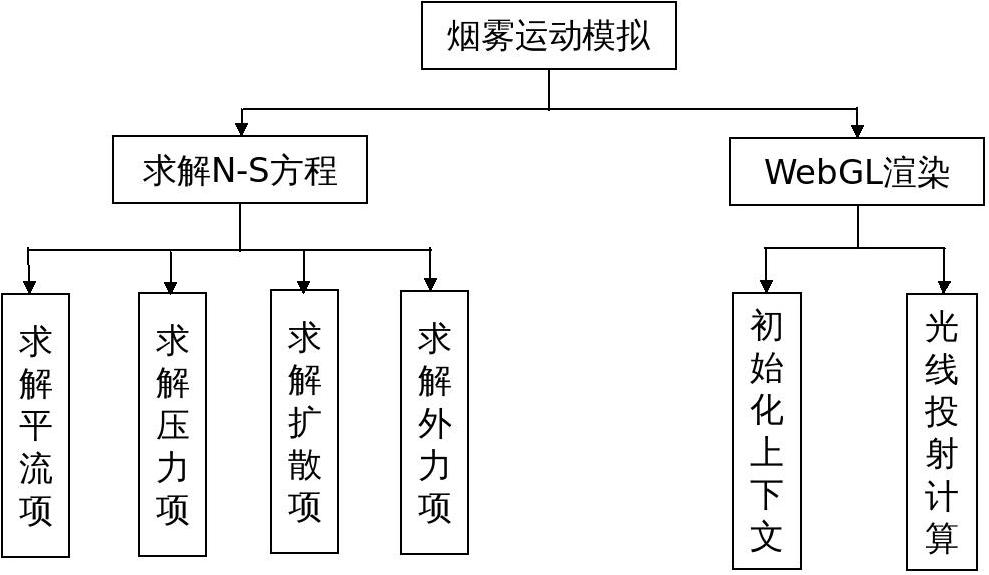
\includegraphics[width=300pt]{struct.jpeg}
\caption{本系统结构图} \label{fig:struct}
\end{figure}

各个模块的主要职责如下:

\begin{itemize}
  \item N-S方程求解模块:主要负责XXX。
  \item WebGL控制模块:主要负责YYY。
\end{itemize}

概要设计的第一个小标题应该是整个论文设计系统的架构,并附上结构图。

\section{本章小结}

除了绪论,每章的最后一节都必须有本章小结,这是学校的规定。